\begin{figure}[t]
    \centering
    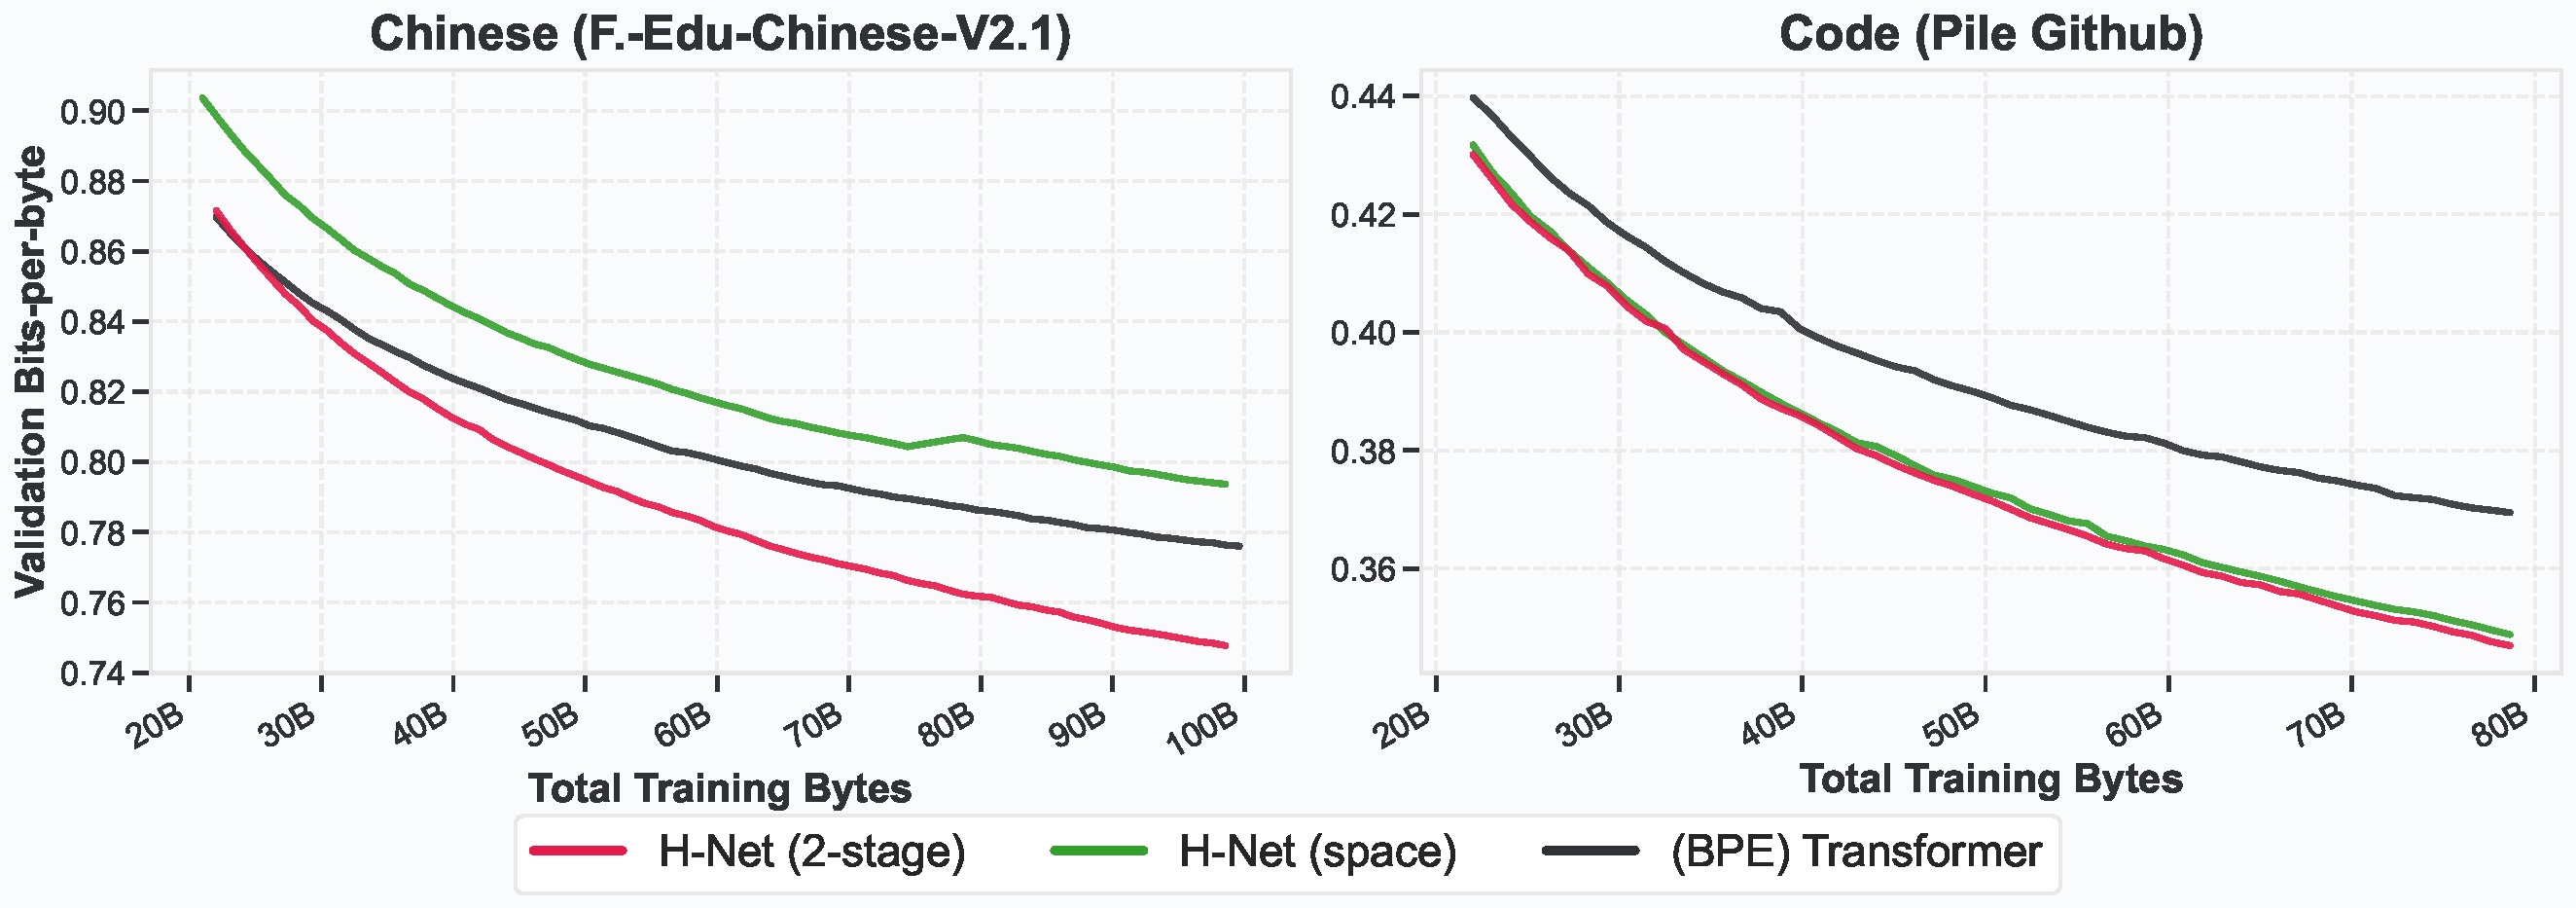
\includegraphics[width=1.0\linewidth]{fig_img/bpb_chinese_code.pdf}
    \caption{
        \textbf{Validation Bits-per-byte (BPB) throughout training on Chinese language and code modeling.}
        \model{} (space) and \model{} (2-stage) are byte-level, while the Transformers use the Llama-3 tokenizer which was designed for multilingual.
        \model{} clearly outperforms both Transformer and \model{} (space) on Chinese language modeling, which does not have space-like segmentation cues, with lower BPB than \model{} (space) throughout training and crossing over with Transformer after around 25B bytes. On code, both \model{} (2-stage) and H-Net (space) significantly outperform BPE Transformer.
        Final post-decay results can be found in \cref{tab: cd-supp}.
    }
    
    \label{fig: bpb_alt_text}
\end{figure}
